\documentclass[12pt,a4paper]{article}
\usepackage[utf8]{inputenc} % sempre salve seus arquivos como UTF8
\usepackage[T1]{fontenc}
\usepackage[english]{babel}

\usepackage[left=2.5cm,right=2cm,top=2cm,bottom=2.5cm]{geometry}
\usepackage{amsmath}
\usepackage{amsthm}
\usepackage{amsfonts}

\usepackage{graphicx}
\usepackage{algorithm}
\usepackage{color}
\usepackage[noend]{algpseudocode}
\usepackage{mathtools}
\usepackage{subfig}
\usepackage{diagbox}

% load times font
\usepackage{mathptmx}
\usepackage[scaled=.90]{helvet}
\usepackage{courier}

% comandos
\newcommand{\mdc}[1]{\mathrm{mdc}(#1)}

\DeclarePairedDelimiter\ceil{\lceil}{\rceil}
\DeclarePairedDelimiter\floor{\lfloor}{\rfloor}

% Foot without marker
\newcommand\blfootnote[1]{%
	\begingroup
	\renewcommand\thefootnote{}\footnote{#1}%
	\addtocounter{footnote}{-1}%
	\endgroup
}

\title{MO446 -- Introduction to Computer Vision  \\ Project 4}
\author{Breno Leite  \\ Guilherme Leite}
\date{26/10/2017}

\begin{document}

\maketitle
\blfootnote{\textit{\textbf{Important note:} The borders seen in the figures are not part of the image, they are figurative information about the starting and ending points of the image. Moreover, all the image scales in this report were changed in order to make the text more readable.}} \\

%% ---------------- Starts here --------------------------------

\textbf{\LARGE Question 3 - Image Descriptor}\\

	In this question we extracted the descriptor of all the images in the data set and saved these descriptors in a file, so the next time the program was executed it could load the descriptors, and perform faster, instead of recalculating every descriptor again.

	An image descriptor consist of all the regions in an image and their information. To extract all regions in an image, firstly we used OpenCV's implementation of the Kmeans algorithm, check Figure \ref{fig:kmeans}.

\newpage

\begin{figure}[!h]
	\centering
	\subfloat[K = 2 regions (colours).]{
		{
			\setlength{\fboxsep}{1pt}
			\setlength{\fboxrule}{1pt}
			\fbox{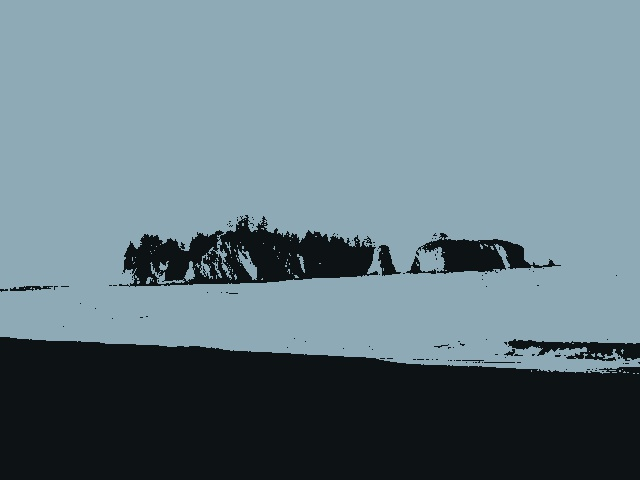
\includegraphics[scale=0.3]{report/p4-3-0-K02}}
		}
		\label{fig:kmeans02}
	}
	\quad
	\subfloat[K = 5 regions (colours).]{
		{
			\setlength{\fboxsep}{1pt}
			\setlength{\fboxrule}{1pt}
			\fbox{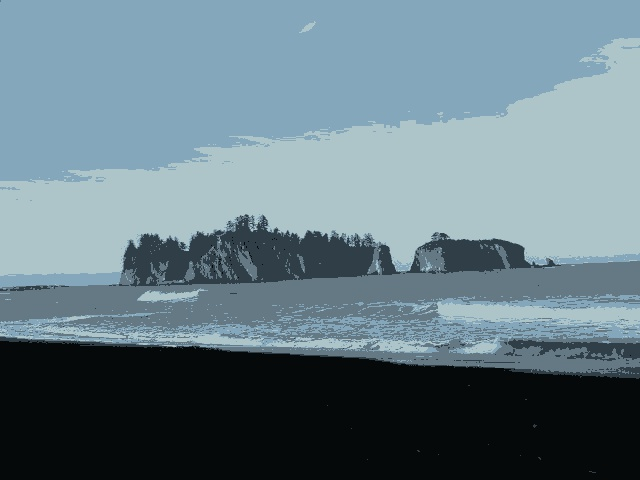
\includegraphics[scale=0.3]{report/p4-3-0-K05}}
		}
		\label{fig:kmeans05}
	}
	\quad
	\subfloat[K = 8 regions (colours).]{
		{
			\setlength{\fboxsep}{1pt}
			\setlength{\fboxrule}{1pt}
			\fbox{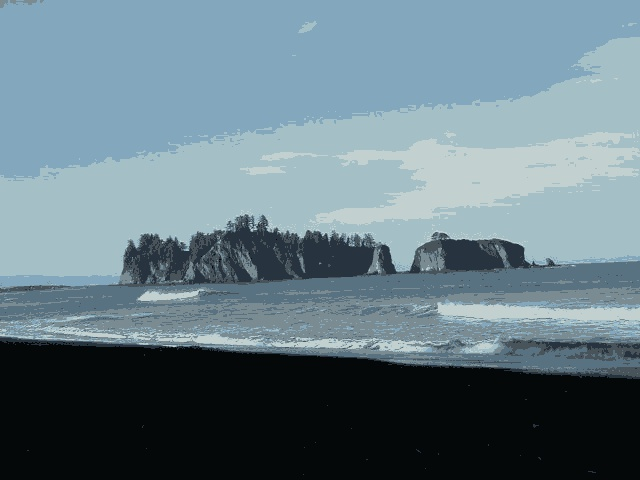
\includegraphics[scale=0.3]{report/p4-3-0-K08}}
		}
		\label{fig:kmeans08}
	}
	\quad
	\subfloat[K = 10 regions (colours).]{
		{
			\setlength{\fboxsep}{1pt}
			\setlength{\fboxrule}{1pt}
			\fbox{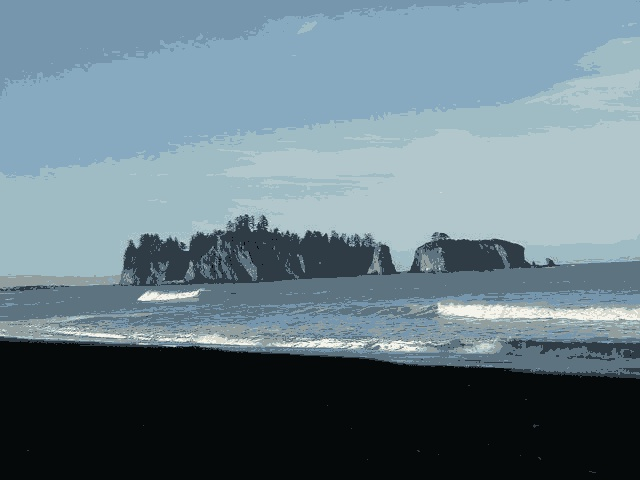
\includegraphics[scale=0.3]{report/p4-3-0-K10}}
		}
		\label{fig:kmeans10}
	}
	\caption{Regions extracted with Kmeans implemented by OpenCV, using different $K$ values.}
	\label{fig:kmeans}
\end{figure}

	The algorithm returns K regions extracted based only in their colours and intensity, in Figure \ref{fig:kmeans} each colour represents a region. The number of regions ($K$) was selected by trial and error, a small $K$ yields big generic regions, in Figure \ref{fig:kmeans02} for example the sky and the ocean were blended into a single region, and that is not helpful to discriminate this image, in contrast a big $K$ yields many small regions as seen in Figure \ref{fig:kmeans10},  too small regions don't really increase the matching accuracy, the reason will be explained later on, although they increase the computation time significantly. The best results for the images analysed were yielded by a value of $K = 5$ regions, seen in Figure \ref{fig:kmeans05}.

	One example of why $K = 5$ is better is the comparison between the sky in Figure \ref{fig:kmeans05} and Figure \ref{fig:kmeans08}, in the former it is possible to distinguish around two colours for the sky region, a light and a dark blue, as in the later the sky was sub-divided into roughly three regions, but a pixel by pixel analysis reveals more regions that won't really improve the matching process, the reason will be explained later on.

	The ideal $K$ value can vary from image to image, and there is a method to minimise between the tested values using silhouette analysis. As in this project the $K$ value was set based on empirical evidence extracted from the data set distributed by the proponent.

	In order to use these regions as an image descriptor, each region has to be descriptive enough to highlight its features. The regions returned by Kmeans are still too generic, some of them are even disconnected into clusters in opposite corners of the image, as in Figure \ref{fig:kmeans05} the sky and some waves posses the same colours and so are seen as the same region, even though they are disconnected and represent different things in the image.

\newpage

\begin{figure}[!h]
	\centering
	\subfloat[K = 2.]{
		{
			\setlength{\fboxsep}{1pt}
			\setlength{\fboxrule}{1pt}
			\fbox{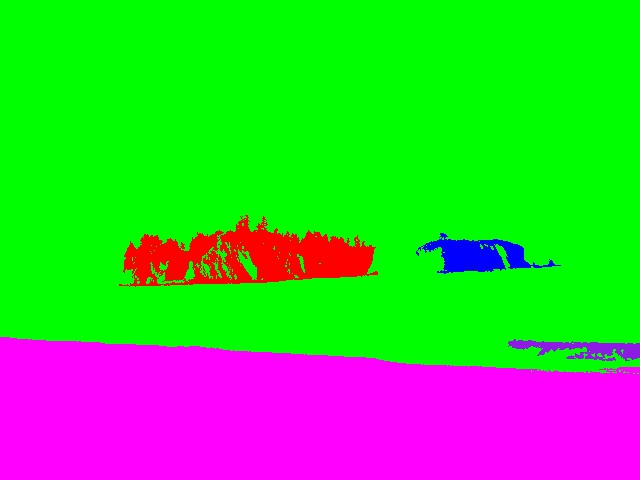
\includegraphics[scale=0.3]{report/p4-3-1-K02}}
		}
		\label{fig:bfs02}
	}
	\quad
	\subfloat[K = 5.]{
		{
			\setlength{\fboxsep}{1pt}
			\setlength{\fboxrule}{1pt}
			\fbox{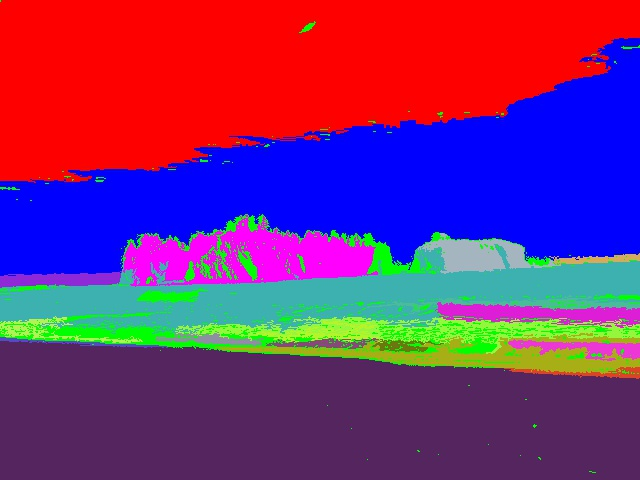
\includegraphics[scale=0.3]{report/p4-3-1-K05}}
		}
		\label{fig:bfs05}
	}
	\quad
	\subfloat[K = 8.]{
		{
			\setlength{\fboxsep}{1pt}
			\setlength{\fboxrule}{1pt}
			\fbox{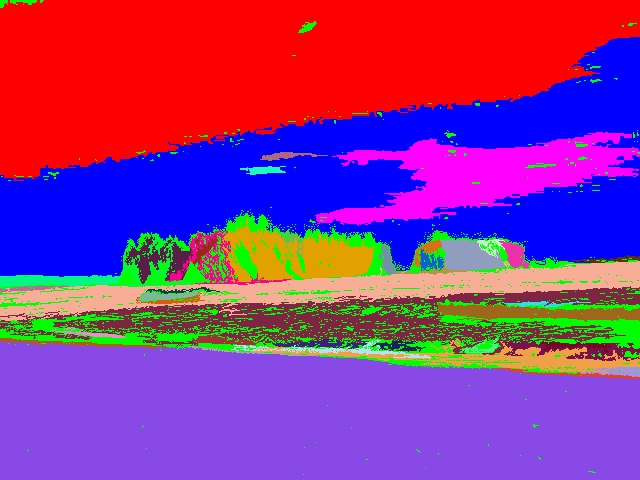
\includegraphics[scale=0.3]{report/p4-3-1-K08}}
		}
		\label{fig:bfs08}
	}
	\quad
	\subfloat[K = 10.]{
		{
			\setlength{\fboxsep}{1pt}
			\setlength{\fboxrule}{1pt}
			\fbox{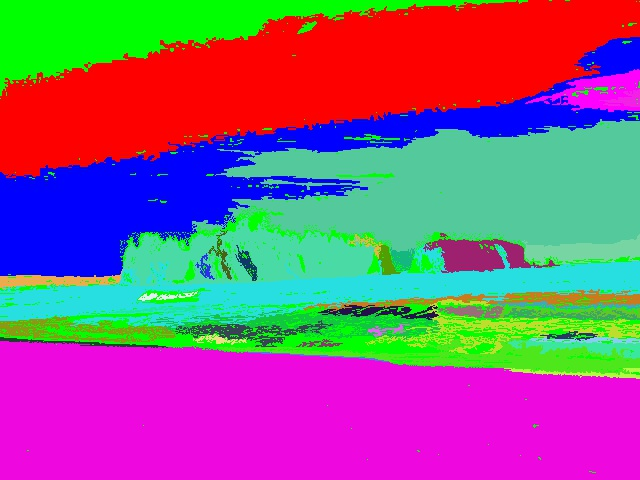
\includegraphics[scale=0.3]{report/p4-3-1-K10}}
		}
		\label{fig:bfs10}
	}
	\caption{Connected regions extracted using the BFS explorer for different $K$ values.}
	\label{fig:bfs}
\end{figure}

	To eliminate these disconnected regions we ran a BFS explorer in the entire image. The BFS returns every connected region, which receives a new label, eliminating disconnected regions altogether. In Figure \ref{fig:bfs} each colour represents a connected region. Regions that are too small don't really describe enough of a feature to be relevant, and thus are discarded, in Figure \ref{fig:bfs} the white colour is used to represent the discarded regions.

	A region is considered too small if its size is smaller than the average of all regions sizes multiplied by a factor of $X$, this value was chosen based on our analysis of the yielded results given by the input data set. In Figure \ref{fig:bfs00} the value of $X$ is set to zero and it is possible to observe regions as big as one pixel being taken, which is counter productive towards our goal.

	The regions returned by Kmeans are based on the intensity of the colours, which means that it is possible that two regions of the same colour and intensity are in opposite corners of the image, disconnected from each other. In order to extract the most expressive features from the image it was necessary to split these cases described above into two or more regions, and to achieve this we used a BFS, as seen in Figure \ref{fig:bfs}, to explore all K regions and create new labels if a region was disconnected. We didn't change the regions boundaries, but doing so would reduce the noise on their borders, leading to better descriptors later on.

	The regions will be used as descriptor of the query image, and to do so we extracted some informations describing each region, we extracted the recommended informations: size of regions, mean colour, centroid and bounding box, and also regarding the texture features we got contrast, correlation and entropy as recommended and also included dissimilarity and energy of the neighbourhood. All the texture features were calculating in an image patch limited by the bounding box of the region, the bounding boxes can be seen in Figure \ref{fig:bbox}.

\begin{figure}[!h]
	\centering
		{
			\setlength{\fboxsep}{1pt}
			\setlength{\fboxrule}{1pt}
			\fbox{\includegraphics[scale=0.5]{output/p4-3-2}}
		}
	\caption{Bounding boxes of the regions \textbf{(p4-3-2)}.}
	\label{fig:bbox}
\end{figure}

% =========================================================================================================================================================

\end{document}
